\documentclass[12pt,a4paper]{article}
\usepackage[a4paper, margin=0.8in, headheight=14pt]{geometry}
\usepackage{fontspec}
\usepackage{unicode-math}
\setmainfont{TeX Gyre Pagella}
\setmonofont[Scale=0.88]{TeX Gyre Cursor}
\setmathfont{Latin Modern Math}
\usepackage{xcolor}
\usepackage{colortbl}
\usepackage{titlesec}
\usepackage{enumitem}
\usepackage{tabularx}
\usepackage{booktabs}
\usepackage{array}
\usepackage{amsmath}
\usepackage{tikz}
\usetikzlibrary{shapes.geometric, arrows.meta, positioning, calc, fit}
\usepackage{tcolorbox}
\tcbuselibrary{skins, breakable}
\usepackage{hyperref}
\usepackage{fancyhdr}
\usepackage{graphicx}
\usepackage{microtype}
\hyphenpenalty=10000
\exhyphenpenalty=10000
\sloppy
\usepackage{caption}
\usepackage{setspace}
\usepackage{multirow}
\usepackage{tocloft}
\newcommand{\Q}[1]{\textbf{#1}\par\noindent\ignorespaces}
\definecolor{myred}{RGB}{196,30,58}
\definecolor{mydark}{RGB}{30,30,50}
\definecolor{mygreen}{RGB}{14,120,80}
\definecolor{myteal}{RGB}{0,130,140}
\definecolor{myamber}{RGB}{180,100,0}
\definecolor{mypurple}{RGB}{100,30,160}
\definecolor{mygray}{RGB}{246,247,249}
\definecolor{mgframe}{RGB}{180,185,200}
\definecolor{watermark}{RGB}{145,150,170}
\definecolor{hdrred}{RGB}{250,232,235}
\definecolor{hdrgreen}{RGB}{220,244,233}
\definecolor{hdrteal}{RGB}{220,242,244}
\definecolor{hdramber}{RGB}{253,242,215}
\definecolor{hdrpurple}{RGB}{238,228,255}
\definecolor{hdrgray}{RGB}{238,240,245}
\definecolor{rowalt}{RGB}{250,251,253}
\titleformat{\section}{\large\bfseries\color{myred}}{\thesection.}{0.5em}{}
  [\vspace{1pt}{\color{myred}\rule{\linewidth}{0.8pt}}]
\titleformat{\subsection}{\normalsize\bfseries\color{myteal}}{\thesubsection}{0.5em}{}
\titlespacing*{\section}{0pt}{18pt}{7pt}
\titlespacing*{\subsection}{0pt}{11pt}{4pt}
\setlength{\parindent}{0pt}
\setlength{\parskip}{4pt}
\renewcommand{\cfttoctitlefont}{\large\bfseries\color{myred}}
\renewcommand{\cftaftertoctitle}{\par\noindent{\color{myred}\rule{\linewidth}{0.8pt}}}
\setlength{\cftbeforetoctitleskip}{0pt}
\setlength{\cftaftertoctitleskip}{6pt}
\renewcommand{\cftsecfont}{\normalsize\bfseries\color{mydark}}
\renewcommand{\cftsecpagefont}{\normalsize\bfseries\color{mydark}}
\renewcommand{\cftsecleader}{\cftdotfill{\cftdotsep}}
\setlength{\cftbeforesecskip}{7pt}
\renewcommand{\cftsubsecfont}{\small\color{mydark}}
\renewcommand{\cftsubsecpagefont}{\small\color{mydark}}
\setlength{\cftbeforesubsecskip}{3pt}
\setlength{\cftsubsecindent}{1.4em}
\renewcommand{\arraystretch}{1.45}
\setlength{\tabcolsep}{6pt}
\arrayrulecolor{mydark}
\newcolumntype{B}[1]{>{\small\bfseries\raggedright\arraybackslash}m{#1}}
\renewcommand{\tabularxcolumn}[1]{m{#1}}
\pagestyle{fancy}\fancyhf{}
\fancyhead[L]{\small\color{myred}\textbf{EC601}\;\color{mydark}--- Control System}
\fancyhead[R]{\small\color{myteal}\textbf{Module 7 Notes}}
\fancyfoot[C]{\small\color{mydark}\thepage}
\fancyfoot[R]{\small\color{watermark}\textit{\copyright\ Biraj}}
\renewcommand{\headrulewidth}{0.5pt}
\renewcommand{\footrulewidth}{0.3pt}
\hypersetup{colorlinks=true,linkcolor=myteal,urlcolor=myteal,
  pdfauthor={Biraj Sarkar},pdftitle={EC601 --- Module 7 Notes}}
\tcbset{
  tikzbox/.style={colback=mygray,colframe=mgframe,boxrule=0.6pt,arc=4pt,
    left=8pt,right=8pt,top=6pt,bottom=6pt,colbacktitle=mgframe,coltitle=mydark,fonttitle=\small\bfseries},
  defbox/.style={colback=hdrgreen,colframe=mygreen,boxrule=0.8pt,arc=4pt,
    left=9pt,right=9pt,top=6pt,bottom=6pt,colbacktitle=mygreen,coltitle=white,fonttitle=\small\bfseries},
  formulabox/.style={colback=hdrteal,colframe=myteal,boxrule=0.8pt,arc=4pt,
    left=9pt,right=9pt,top=7pt,bottom=7pt,colbacktitle=myteal,coltitle=white,fonttitle=\small\bfseries},
  examplebox/.style={colback=hdramber,colframe=myamber,boxrule=0.8pt,arc=4pt,
    left=9pt,right=9pt,top=6pt,bottom=6pt,colbacktitle=myamber,coltitle=white,fonttitle=\small\bfseries},
  masonbox/.style={colback=hdrpurple,colframe=mypurple,boxrule=0.8pt,arc=4pt,
    left=9pt,right=9pt,top=6pt,bottom=6pt,colbacktitle=mypurple,coltitle=white,fonttitle=\small\bfseries},
  exambox/.style={colback=hdrpurple,colframe=mypurple,boxrule=1pt,arc=5pt,
    left=10pt,right=10pt,top=8pt,bottom=8pt,colbacktitle=mypurple,coltitle=white,fonttitle=\bfseries, breakable, title after break={\textbf{Frequently Asked / Viva Questions (contd.)}}}
}
% Allow all boxes to break across pages
\tcbset{breakable}
\tikzset{
  block/.style={rectangle,draw=myteal,fill=hdrteal,text width=2.4cm,align=center,
    minimum height=0.9cm,font=\small,rounded corners=3pt,line width=0.7pt},
  wblock/.style={rectangle,draw=myteal,fill=hdrteal,text width=3.2cm,align=center,
    minimum height=0.9cm,font=\small,rounded corners=3pt,line width=0.7pt},
  redblock/.style={rectangle,draw=myred,fill=hdrred,text width=2.4cm,align=center,
    minimum height=0.9cm,font=\small,rounded corners=3pt,line width=0.7pt},
  sumjunc/.style={circle,draw=myamber,fill=hdramber,minimum size=0.62cm,font=\small,line width=0.8pt},
  arrow/.style={-Stealth,thick,color=mydark},
  redarrow/.style={-Stealth,thick,color=myred},
  line/.style={thick,color=mydark}
}
\begin{document}
\begin{center}
  {\LARGE\bfseries\color{myred} EC601 --- Control System}\\[5pt]
  {\normalsize\color{mydark} Semester VI \quad$\bullet$\quad 3L:0T:0P \quad$\bullet$\quad 3 Credits}\\[3pt]
  {\normalsize\color{myteal}\textbf{Module 7 Exam Notes}}\\[3pt]
  {\small\color{mydark} CGEC \;$|$\; B.Tech ECE (2023--27) \;$|$\; \textit{Biraj Sarkar}}
\end{center}
\vspace{2pt}\noindent{\color{myred}\rule{\linewidth}{1.5pt}}\vspace{2pt}
\hypersetup{linkcolor=mydark}
\tableofcontents
\hypersetup{linkcolor=myteal}\newpage

%═══════════════════════════════════════════════════════════════════════════════
\section{Cathode Ray Oscilloscope (CRO)}
%═══════════════════════════════════════════════════════════════════════════════

\begin{tcolorbox}[defbox]
\textbf{CRO (Cathode Ray Oscilloscope):} An electronic test instrument that displays electrical signals as waveforms on a phosphor screen. It plots voltage (Y-axis) vs time (X-axis) in real time, allowing measurement of amplitude, frequency, phase, rise time, and waveform shape.
\end{tcolorbox}

\subsection{Block Diagram of CRO}

\begin{tcolorbox}[tikzbox, title={CRO Block Diagram}]
\centering
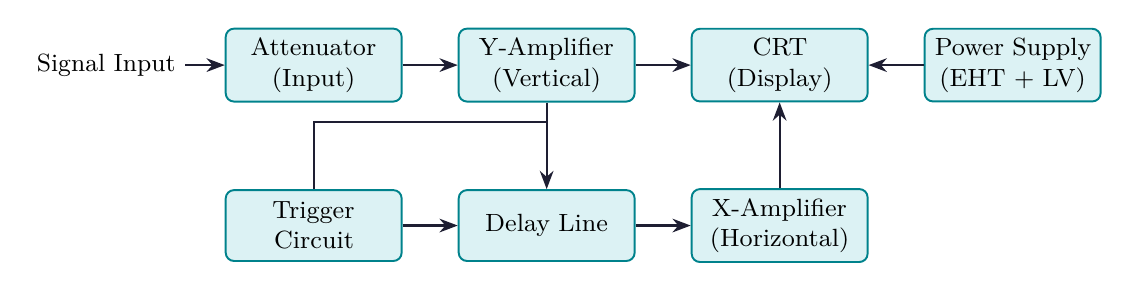
\begin{tikzpicture}[node distance=0.4cm and 0.7cm,
  sblock/.style={rectangle, draw=myteal, fill=hdrteal, text width=2.0cm,
    align=center, minimum height=0.9cm, font=\small, rounded corners=3pt, line width=0.7pt}]

  % ── Top row (left to right): Attenuator → Y-Amp → CRT ──────────────────
  \node[sblock] (atten) {Attenuator\\(Input)};
  \node[sblock, right=0.7cm of atten] (yamp)  {Y-Amplifier\\(Vertical)};
  \node[sblock, right=0.7cm of yamp]  (crt)   {CRT\\(Display)};
  \node[sblock, right=0.7cm of crt]   (psu)   {Power Supply\\(EHT + LV)};

  % ── Bottom row: Trigger → Delay → X-Amp ────────────────────────────────
  \node[sblock, below=1.1cm of atten] (trig)  {Trigger\\Circuit};
  \node[sblock, right=0.7cm of trig]  (delay) {Delay Line};
  \node[sblock, right=0.7cm of delay] (xamp)  {X-Amplifier\\(Horizontal)};

  % ── Signal path ─────────────────────────────────────────────────────────
  \draw[arrow] (atten) -- (yamp);
  \draw[arrow] (yamp)  -- (crt);
  \draw[arrow] (psu)   -- (crt);

  % ── Sweep path ──────────────────────────────────────────────────────────
  \draw[arrow] (trig)  -- (delay);
  \draw[arrow] (delay) -- (xamp);
  \draw[arrow] (xamp)  -- (crt);

  % ── Y-amp → Delay Line (vertical tap) ───────────────────────────────────
  \draw[arrow] (yamp.south) -- (delay.north);

  % ── Trigger tapped from Y-amp ────────────────────────────────────────────
  \coordinate (ytap) at ($(yamp.south)+(0,-0.25)$);
  \draw[line]  (ytap) -| (trig.north);

  % ── Input label ──────────────────────────────────────────────────────────
  \node[left=0.5cm of atten, font=\small] {Signal Input};
  \draw[arrow] ($(atten.west)-(0.5,0)$) -- (atten.west);
\end{tikzpicture}
\end{tcolorbox}

\subsection{Main Blocks and Functions}

\begin{tabularx}{\linewidth}{|B{3.2cm}|X|}
\hline
\multicolumn{1}{|>{\centering\arraybackslash}m{3.2cm}|}{\textbf{\color{myteal}Block}} &
\multicolumn{1}{>{\centering\arraybackslash}X|}{\textbf{\color{myteal}Function}} \\
\hline
Attenuator & Reduces input signal to a safe level for the amplifier. Calibrated in V/div. \\
\hline
Y-Amplifier & Amplifies the vertical (signal) input to drive the vertical deflection plates of CRT. \\
\hline
Delay Line & Delays the signal slightly so the sweep starts before the signal arrives --- ensures complete waveform display. \\
\hline
Trigger Circuit & Synchronises the sweep with the input signal to produce a stable display. \\
\hline
Time Base (Sweep Gen.) & Generates a sawtooth waveform for horizontal deflection. Calibrated in time/div. \\
\hline
X-Amplifier & Amplifies the time base signal to drive the horizontal deflection plates. \\
\hline
CRT & Cathode Ray Tube --- electron gun, deflection plates, phosphor screen. Displays the waveform. \\
\hline
Power Supply & Provides EHT ($\sim$1--10 kV) for CRT and low voltages for amplifiers. \\
\hline
\end{tabularx}

\subsection{Measurements with CRO}

\begin{tabularx}{\linewidth}{|B{3.0cm}|X|}
\hline
\multicolumn{1}{|>{\centering\arraybackslash}m{3.0cm}|}{\textbf{\color{mygreen}Measurement}} &
\multicolumn{1}{>{\centering\arraybackslash}X|}{\textbf{\color{mygreen}Method}} \\
\hline
Voltage (peak) & Count vertical divisions $\times$ V/div setting. $V_{pk} = n_{div} \times \text{V/div}$ \\
\hline
Time period $T$ & Count horizontal divisions for one cycle $\times$ time/div. $T = n_{div} \times \text{time/div}$ \\
\hline
Frequency & $f = 1/T$ \\
\hline
Phase difference & Use dual-trace mode; measure time shift $\Delta t$. $\phi = (\Delta t / T)\times 360°$ \\
\hline
Rise time & Time for signal to go from 10\% to 90\% of final value. \\
\hline
DC voltage & Set coupling to DC; measure vertical displacement from zero. \\
\hline
\end{tabularx}

\subsection{Lissajous Figures (Phase \& Frequency Measurement)}

Lissajous figures are patterns displayed on a CRO screen when two sinusoidal signals of different or same frequencies are applied simultaneously to the horizontal ($X$) and vertical ($Y$) deflection plates. They are used to measure \textbf{phase difference} and \textbf{frequency ratio}.

\begin{tcolorbox}[defbox, title={Phase Difference Measurement}]
When two sine waves of equal frequency ($f_x = f_y$) but different phase are applied, the pattern is an \textbf{ellipse}. The phase difference $\theta$ is calculated from the intercepts:
$$\sin\theta \;=\; \frac{y_1}{y_2} \quad\Rightarrow\quad \theta \;=\; \sin^{-1}\!\!\left(\frac{y_1}{y_2}\right) \quad \text{or} \quad 180^\circ - \sin^{-1}\!\!\left(\frac{y_1}{y_2}\right)$$
where $y_1$ is the y-intercept (height at $x=0$) and $y_2$ is the maximum vertical deflection.
\end{tcolorbox}

\begin{tcolorbox}[tikzbox, title={Lissajous Phase Ellipse}]
\centering
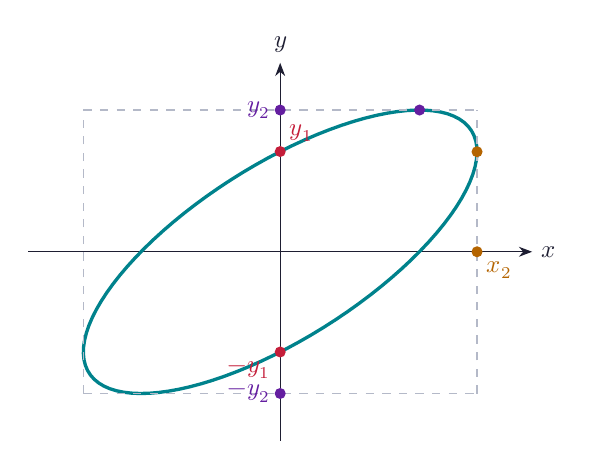
\begin{tikzpicture}[scale=1.0]
  % Axes
  \draw[-Stealth, thin, color=mydark] (-3.2,0) -- (3.2,0) node[right]{\small $x$};
  \draw[-Stealth, thin, color=mydark] (0,-2.4) -- (0,2.4) node[above]{\small $y$};
  
  % Ellipse (A_x = 2.5, A_y = 1.8, phase = 45 degrees)
  \draw[line width=1.2pt, color=myteal, domain=0:360, samples=100] 
    plot ({2.5*sin(\x)}, {1.8*sin(\x + 45)});
  
  % y-intercept y_1
  \fill[myred] (0, {1.8*sin(45)}) circle (2pt) node[above right, color=myred]{\small $y_1$};
  \fill[myred] (0, {-1.8*sin(45)}) circle (2pt) node[below left, color=myred]{\small $-y_1$};
  
  % maximum height y_2
  \draw[dashed, color=mgframe] (-2.5, 1.8) -- (2.5, 1.8);
  \draw[dashed, color=mgframe] (-2.5, -1.8) -- (2.5, -1.8);
  \fill[mypurple] (1.77, 1.8) circle (2pt);
  \fill[mypurple] (0, 1.8) circle (2pt) node[left, color=mypurple]{\small $y_2$};
  \fill[mypurple] (0, -1.8) circle (2pt) node[left, color=mypurple]{\small $-y_2$};
  
  % horizontal maximum x_2
  \draw[dashed, color=mgframe] (2.5, -1.8) -- (2.5, 1.8);
  \draw[dashed, color=mgframe] (-2.5, -1.8) -- (-2.5, 1.8);
  \fill[myamber] (2.5, 1.27) circle (2pt);
  \fill[myamber] (2.5, 0) circle (2pt) node[below right, color=myamber]{\small $x_2$};
\end{tikzpicture}
\end{tcolorbox}

\begin{tcolorbox}[defbox, title={Frequency Measurement}]
If the frequencies are unequal, the frequency ratio is determined by drawing a horizontal and a vertical line through the pattern and counting the number of tangency points:
$$\frac{f_y}{f_x} \;=\; \frac{\text{Number of Horizontal Tangencies } (N_h)}{\text{Number of Vertical Tangencies } (N_v)}$$
\end{tcolorbox}

\subsection{Special Purpose Oscilloscopes: Dual-Trace vs. Dual-Beam \& DSO}

Modern electronic testing requires displaying multiple signals simultaneously and storing waveforms for analysis.

\subsubsection{Dual-Trace vs. Dual-Beam Oscilloscopes}

\begin{tabularx}{\linewidth}{|B{2.8cm}|X|X|}
\hline
\multicolumn{1}{|>{\centering\arraybackslash}m{2.8cm}|}{\textbf{Parameter}} &
\multicolumn{1}{>{\centering\arraybackslash}X|}{\textbf{\color{myteal}Dual-Trace CRO}} &
\multicolumn{1}{>{\centering\arraybackslash}X|}{\textbf{\color{myamber}Dual-Beam CRO}} \\
\hline
Electron Gun & Single electron gun. & Two separate electron guns (or split beam with two deflection systems). \\
\hline
Deflection System & One set of vertical deflection plates. & Two independent sets of vertical deflection plates. \\
\hline
Working Method & Uses electronic switching (Chop or Alternate mode) to display two traces. & Displays two signals simultaneously by writing with two separate beams. \\
\hline
Modes & \textbf{Chop:} switches channels at high speed (low $f$ signals). \textbf{Alternate:} swaps channel after each sweep (high $f$ signals). & Simpler circuitry; no switching required. \\
\hline
Cost \& Complexity & Moderate cost; standard design. & Highly complex; expensive CRT assembly. \\
\hline
Trace Alignment & Perfect alignment; single electron path. & Beam alignment can drift over time. \\
\hline
\end{tabularx}

\subsubsection{Digital Storage Oscilloscope (DSO)}

A \textbf{Digital Storage Oscilloscope (DSO)} digitises the analog input signal and stores it in digital memory. It then reads this data from memory to reconstruct and display the waveform on the screen.

\begin{tcolorbox}[tikzbox, title={DSO Digitisation Block Diagram}]
\centering
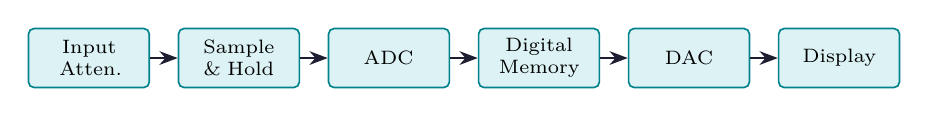
\begin{tikzpicture}[node distance=0.2cm and 0.4cm,
  sblock/.style={rectangle, draw=myteal, fill=hdrteal, text width=1.3cm,
    align=center, minimum height=0.75cm, font=\scriptsize,
    rounded corners=2pt, line width=0.6pt}]
  \node[sblock] (inp) {Input\\Atten.};
  \node[sblock, right=0.35cm of inp] (sh) {Sample\\\& Hold};
  \node[sblock, right=0.35cm of sh] (adc) {ADC};
  \node[sblock, right=0.35cm of adc] (mem) {Digital\\Memory};
  \node[sblock, right=0.35cm of mem] (dac) {DAC};
  \node[sblock, right=0.35cm of dac] (disp) {Display};
  
  \draw[arrow] (inp) -- (sh);
  \draw[arrow] (sh) -- (adc);
  \draw[arrow] (adc) -- (mem);
  \draw[arrow] (mem) -- (dac);
  \draw[arrow] (dac) -- (disp);
\end{tikzpicture}
\end{tcolorbox}

\begin{itemize}[leftmargin=*, itemsep=3pt]
  \item \textbf{Sample and Hold (S\&H):} Holds the analog voltage constant long enough for the ADC to convert it.
  \item \textbf{ADC (Analog-to-Digital Converter):} Converts the held analog sample into a digital word (binary code).
  \item \textbf{Digital Memory (RAM):} Stores the binary samples sequentially.
  \item \textbf{DAC (Digital-to-Analog Converter):} Converts the stored data back to an analog signal.
  \item \textbf{Display:} Reconstructs and plots the signal.
\end{itemize}

\textbf{Key Advantages of DSO over Analog CRO:}
\begin{enumerate}[label=\textbf{\arabic*.}, leftmargin=*, itemsep=2pt]
  \item \textbf{Infinite Storage Time:} Waveforms are stored in memory and can be held indefinitely.
  \item \textbf{Pre-trigger Viewing:} DSOs can display signals that occurred \textit{before} the trigger point using a circular buffer.
  \item \textbf{Signal Processing:} Direct microprocessor analysis (FFT, peak-to-peak, RMS, frequency).
  \item \textbf{Easy Export:} Stored data can be transferred to a computer.
\end{enumerate}

%═══════════════════════════════════════════════════════════════════════════════
\section{Wave Analyzer and Spectrum Analyzer}
%â• â• â• â• â• â• â• â• â• â• â• â• â• â• â• â• â• â• â• â• â• â• â• â• â• â• â• â• â• â• â• â• â• â• â• â• â• â• â• â• â• â• â• â• â• â• â• â• â• â• â• â• â• â• â• â• â• â• â• â• â• â• â• â• â• â• â• â• â• â• â• â• â• â• â• â• â• â• â• 

\subsection{Wave Analyzer}

\begin{tcolorbox}[defbox]
\textbf{Wave Analyzer:} An instrument that measures the \textbf{amplitude} and \textbf{frequency} of individual harmonic components of a complex periodic waveform. It is essentially a \textit{very narrow bandpass filter} that can be tuned to any frequency within its range.
\end{tcolorbox}

\textbf{Requirements:}
\begin{itemize}[leftmargin=*, itemsep=2pt]
  \item Very narrow, stable, and tunable bandpass filter
  \item High selectivity (ability to separate closely spaced harmonics)
  \item High sensitivity (detect small amplitude components)
  \item Calibrated frequency and amplitude readout
\end{itemize}

\begin{tcolorbox}[tikzbox, title={Wave Analyzer Block Diagram}]
\centering
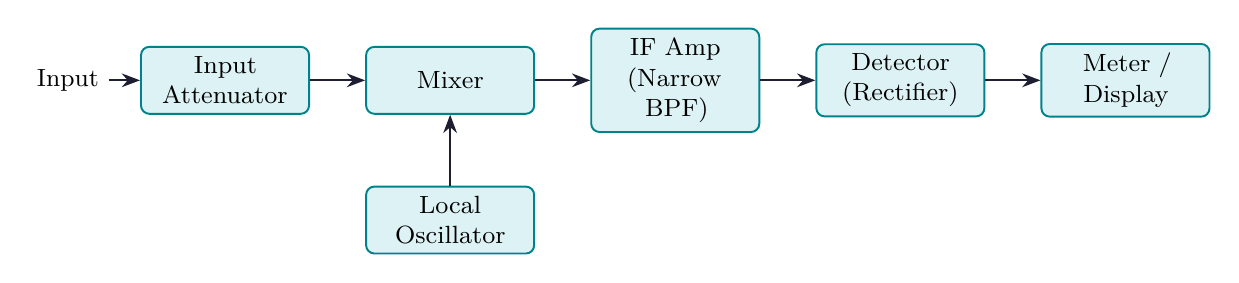
\begin{tikzpicture}[node distance=0.3cm and 0.7cm,
  sblock/.style={rectangle, draw=myteal, fill=hdrteal, text width=1.9cm,
    align=center, minimum height=0.85cm, font=\small, rounded corners=3pt, line width=0.7pt}]
  \node[sblock] (inp)   {Input\\Attenuator};
  \node[sblock, right=0.7cm of inp]   (mixer) {Mixer};
  \node[sblock, right=0.7cm of mixer] (if)    {IF Amp\\(Narrow BPF)};
  \node[sblock, right=0.7cm of if]    (det)   {Detector\\(Rectifier)};
  \node[sblock, right=0.7cm of det]   (meter) {Meter /\\Display};
  \node[sblock, below=0.9cm of mixer] (osc)   {Local\\Oscillator};

  \draw[arrow] (inp) -- (mixer);
  \draw[arrow] (mixer) -- (if);
  \draw[arrow] (if) -- (det);
  \draw[arrow] (det) -- (meter);
  \draw[arrow] (osc) -- (mixer);
  \node[left=0.4cm of inp, font=\small] {Input};
  \draw[arrow] ($(inp.west)-(0.4,0)$) -- (inp.west);
\end{tikzpicture}
\end{tcolorbox}

\subsection{Spectrum Analyzer}

\begin{tcolorbox}[defbox]
\textbf{Spectrum Analyzer:} Displays the \textbf{frequency spectrum} of a signal --- amplitude (or power) vs frequency. Unlike the wave analyzer (which measures one frequency at a time), the spectrum analyzer displays \textit{all frequency components simultaneously} on a screen (frequency domain display).
\end{tcolorbox}

\textbf{Requirements:}
\begin{itemize}[leftmargin=*, itemsep=2pt]
  \item Wide frequency range with fine resolution
  \item High dynamic range (detect weak signals near strong ones)
  \item Fast sweep speed for real-time display
  \item Calibrated frequency (X-axis) and amplitude/power (Y-axis in dBm)
\end{itemize}

\begin{tcolorbox}[tikzbox, title={Spectrum Analyzer Block Diagram (Swept Superheterodyne)}]
\centering
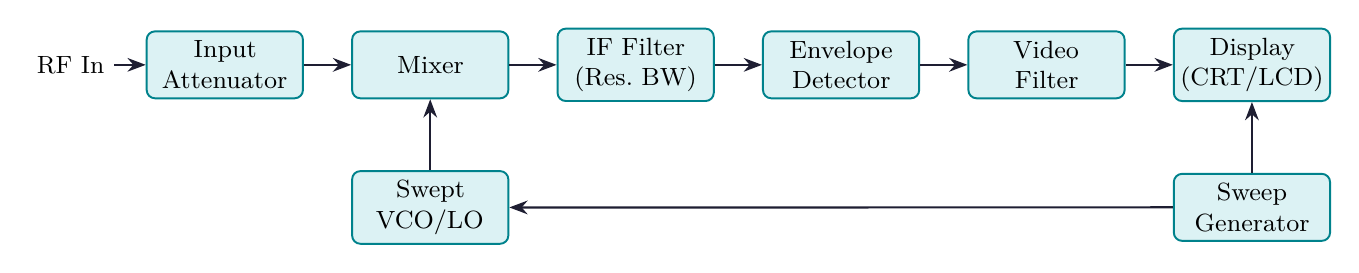
\begin{tikzpicture}[node distance=0.3cm and 0.65cm,
  sblock/.style={rectangle, draw=myteal, fill=hdrteal, text width=1.75cm,
    align=center, minimum height=0.85cm, font=\small, rounded corners=3pt, line width=0.7pt}]
  \node[sblock] (inp)  {Input\\Attenuator};
  \node[sblock, right=0.6cm of inp]  (mix)  {Mixer};
  \node[sblock, right=0.6cm of mix]  (if)   {IF Filter\\(Res.\ BW)};
  \node[sblock, right=0.6cm of if]   (det)  {Envelope\\Detector};
  \node[sblock, right=0.6cm of det]  (vbw)  {Video\\Filter};
  \node[sblock, right=0.6cm of vbw]  (disp) {Display\\(CRT/LCD)};
  \node[sblock, below=0.9cm of mix]  (vco)  {Swept\\VCO/LO};
  \node[sblock, below=0.9cm of disp] (sweep){Sweep\\Generator};

  \draw[arrow] (inp)  -- (mix);
  \draw[arrow] (mix)  -- (if);
  \draw[arrow] (if)   -- (det);
  \draw[arrow] (det)  -- (vbw);
  \draw[arrow] (vbw)  -- (disp);
  \draw[arrow] (vco)  -- (mix);
  \draw[arrow] (sweep)-- (vco);
  \draw[arrow] (sweep)-- (disp);
  \node[left=0.4cm of inp, font=\small] {RF In};
  \draw[arrow] ($(inp.west)-(0.4,0)$) -- (inp.west);
\end{tikzpicture}
\end{tcolorbox}

\begin{tabularx}{\linewidth}{|B{3.0cm}|>{\centering\arraybackslash}X|>{\centering\arraybackslash}X|}
\hline
\multicolumn{1}{|>{\centering\arraybackslash}m{3.0cm}|}{\textbf{Feature}} &
\textbf{\color{myamber}Wave Analyzer} & \textbf{\color{mygreen}Spectrum Analyzer} \\
\hline
Display & One frequency at a time & All frequencies simultaneously \\
\hline
Domain & Frequency (selective) & Frequency (full spectrum) \\
\hline
Speed & Slow (manual tuning) & Fast (swept or FFT) \\
\hline
Use & Harmonic distortion analysis & Wideband signal analysis \\
\hline
\end{tabularx}

%═══════════════════════════════════════════════════════════════════════════════
\section{LVDT (Linear Variable Differential Transformer)}
%═══════════════════════════════════════════════════════════════════════════════

\begin{tcolorbox}[defbox]
\textbf{LVDT:} A \textbf{Linear Variable Differential Transformer} is an electromechanical transducer that converts linear displacement into a proportional AC voltage. It is the most widely used inductive displacement sensor due to its high accuracy, infinite resolution, and frictionless operation.
\end{tcolorbox}

\subsection{Construction and Working}

\textbf{Construction:} One primary coil (centre) and two secondary coils (S1, S2) wound symmetrically on a cylindrical former. A movable ferromagnetic \textbf{core} (plunger) slides inside without contact.

\textbf{Working:}
\begin{enumerate}[label=\textbf{\arabic*.}, leftmargin=*, itemsep=3pt]
  \item AC excitation applied to primary coil induces EMF in both secondary coils.
  \item Secondary coils connected in \textbf{series opposition}: $V_{out} = V_{S1} - V_{S2}$.
  \item \textbf{Null position} (core centred): $V_{S1} = V_{S2}$, so $V_{out} = 0$.
  \item \textbf{Core displaced right:} $V_{S1} > V_{S2}$, $V_{out}$ is positive and in phase with primary.
  \item \textbf{Core displaced left:} $V_{S2} > V_{S1}$, $V_{out}$ is negative (180° phase shift).
\end{enumerate}

\begin{tcolorbox}[tikzbox, title={LVDT Construction and Output Characteristic}]
\centering
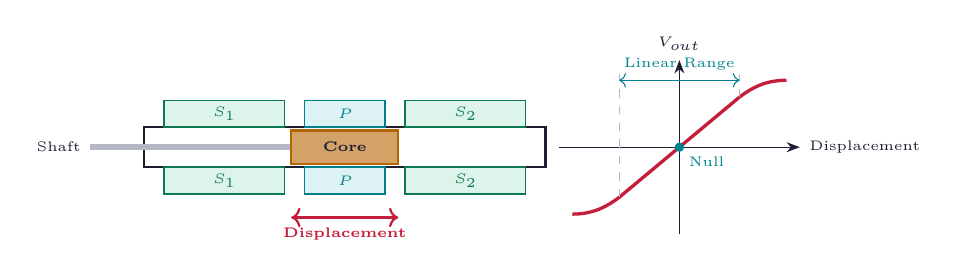
\begin{tikzpicture}[scale=0.85]
  % Former Hollow Shaft
  \draw[line width=0.8pt, color=mydark] (0,0.9) rectangle (6,1.5);
  
  % Shaft/Arm
  \draw[line width=2.0pt, color=mgframe] (2.2,1.2) -- (-0.8,1.2);
  \node[left, font=\tiny, color=mydark] at (-0.8,1.2) {Shaft};
  
  % Core (inside former channel)
  \fill[myamber!60, draw=myamber, line width=0.8pt] (2.2,0.95) rectangle (3.8,1.45);
  \node[font=\tiny\bfseries, color=mydark] at (3.0,1.2) {Core};
  
  % Coils Upper Half (above former)
  \fill[hdrgreen, draw=mygreen, line width=0.6pt] (0.3,1.5) rectangle (2.1,1.9);
  \node[font=\tiny, color=mygreen] at (1.2,1.7) {$S_1$};
  \fill[hdrteal, draw=myteal, line width=0.6pt] (2.4,1.5) rectangle (3.6,1.9);
  \node[font=\tiny, color=myteal] at (3.0,1.7) {$P$};
  \fill[hdrgreen, draw=mygreen, line width=0.6pt] (3.9,1.5) rectangle (5.7,1.9);
  \node[font=\tiny, color=mygreen] at (4.8,1.7) {$S_2$};
  
  % Coils Lower Half (below former)
  \fill[hdrgreen, draw=mygreen, line width=0.6pt] (0.3,0.5) rectangle (2.1,0.9);
  \node[font=\tiny, color=mygreen] at (1.2,0.7) {$S_1$};
  \fill[hdrteal, draw=myteal, line width=0.6pt] (2.4,0.5) rectangle (3.6,0.9);
  \node[font=\tiny, color=myteal] at (3.0,0.7) {$P$};
  \fill[hdrgreen, draw=mygreen, line width=0.6pt] (3.9,0.5) rectangle (5.7,0.9);
  \node[font=\tiny, color=mygreen] at (4.8,0.7) {$S_2$};
  
  % Displacement arrow (bottom)
  \draw[<->, color=myred, thick] (2.2,0.15) -- (3.8,0.15) node[midway, below, font=\tiny\bfseries] {Displacement};
  
  % Output characteristic
  \begin{scope}[xshift=8.0cm, yshift=1.2cm]
    \draw[-Stealth, thin, color=mydark] (-1.8,0) -- (1.8,0) node[right, font=\tiny] {Displacement};
    \draw[-Stealth, thin, color=mydark] (0,-1.3) -- (0,1.3) node[above, font=\tiny] {$V_{out}$};
    
    % Curve with linear range and non-linear ends
    \draw[color=myred, line width=1.2pt] 
      (-1.6,-1.0) .. controls (-1.3,-1.0) and (-1.1,-0.9) .. (-0.9,-0.75)
      -- (0.9,0.75) 
      .. controls (1.1,0.9) and (1.3,1.0) .. (1.6,1.0);
      
    \fill[myteal] (0,0) circle (2pt);
    \node[below right, font=\tiny, color=myteal] at (0,0) {Null};
    
    % Dashed lines marking linear region limits
    \draw[dashed, color=mgframe, thin] (-0.9, -0.75) -- (-0.9, 1.1);
    \draw[dashed, color=mgframe, thin] (0.9, 0.75) -- (0.9, 1.1);
    \draw[<->, color=myteal, thin] (-0.9, 1.0) -- (0.9, 1.0) node[midway, above, font=\tiny] {Linear Range};
  \end{scope}
\end{tikzpicture}
\end{tcolorbox}

\begin{tabularx}{\linewidth}{|>{\centering\arraybackslash}X|>{\centering\arraybackslash}X|}
\hline
\textbf{\color{mygreen}Advantages} & \textbf{\color{myred}Disadvantages} \\
\hline
Infinite resolution (frictionless) & Sensitive to stray magnetic fields \\
\hline
High accuracy and repeatability & Requires AC excitation and demodulator \\
\hline
No mechanical wear (contactless) & Limited to linear displacement \\
\hline
Rugged; works in harsh environments & Bulkier than resistive sensors \\
\hline
\end{tabularx}

%═══════════════════════════════════════════════════════════════════════════════
\section{Servomotors}
%═══════════════════════════════════════════════════════════════════════════════

\begin{tcolorbox}[defbox]
\textbf{Servomotor:} A motor specifically designed for use in \textbf{closed-loop control systems} (servo systems). It must have a linear torque-speed characteristic, low inertia, fast response, and be controllable by an error signal. Used for precise position, speed, or torque control.
\end{tcolorbox}

\subsection{DC Servomotor}

\begin{tcolorbox}[defbox]
\textbf{DC Servomotor:} A DC motor with a separately excited field or permanent magnet field, controlled by varying the \textbf{armature voltage}. The torque is proportional to armature current; speed is proportional to back-EMF.
\end{tcolorbox}

\begin{tcolorbox}[formulabox, title={DC Servomotor Equations}]
\textbf{Electrical:} $V_a = E_b + I_a R_a + L_a \dfrac{dI_a}{dt}$, \quad $E_b = K_b\,\omega$\\[4pt]
\textbf{Mechanical:} $T = K_T\,I_a = J\dfrac{d\omega}{dt} + B\,\omega$\\[4pt]
\textbf{Transfer Function} (armature control, $L_a \approx 0$):
$$\frac{\Omega(s)}{V_a(s)} = \frac{K_T/R_a}{Js + B + K_TK_b/R_a}$$
where $K_T$ = torque constant, $K_b$ = back-EMF constant, $J$ = inertia, $B$ = damping.
\end{tcolorbox}

\begin{tabularx}{\linewidth}{|B{3.0cm}|X|}
\hline
\multicolumn{1}{|>{\centering\arraybackslash}m{3.0cm}|}{\textbf{\color{myteal}Feature}} &
\multicolumn{1}{>{\centering\arraybackslash}X|}{\textbf{\color{myteal}DC Servomotor}} \\
\hline
Control method & Armature voltage control or field control \\
\hline
Torque-speed & Linear (ideal for servo use) \\
\hline
Response & Fast; low inertia rotor \\
\hline
Maintenance & Brushes require periodic replacement \\
\hline
Applications & Robotics, CNC machines, antenna positioning \\
\hline
\end{tabularx}

\subsection{AC Servomotor}

\begin{tcolorbox}[defbox]
\textbf{AC Servomotor:} A two-phase induction motor used in servo systems. One phase (reference phase) is supplied with a fixed AC voltage; the other phase (control phase) receives a variable voltage proportional to the error signal. Speed and direction are controlled by the magnitude and phase of the control voltage.
\end{tcolorbox}

\begin{tcolorbox}[formulabox, title={AC Servomotor Key Features}]
\begin{itemize}[leftmargin=*, itemsep=2pt, topsep=2pt]
  \item \textbf{High rotor resistance:} Ensures stable, linear torque-speed characteristic (negative slope throughout).
  \item \textbf{Low inertia:} Drag-cup or thin-disc rotor for fast response.
  \item \textbf{Control:} Vary amplitude of control phase voltage; direction by phase reversal ($\pm 90°$).
  \item \textbf{Transfer function:} $G(s) = K_m / (s(\tau_m s + 1))$ where $K_m$ = motor gain, $\tau_m$ = mechanical time constant.
\end{itemize}
\end{tcolorbox}

\begin{tabularx}{\linewidth}{|B{3.0cm}|>{\centering\arraybackslash}X|>{\centering\arraybackslash}X|}
\hline
\multicolumn{1}{|>{\centering\arraybackslash}m{3.0cm}|}{\textbf{Feature}} &
\textbf{\color{myamber}DC Servomotor} & \textbf{\color{mygreen}AC Servomotor} \\
\hline
Supply & DC & 2-phase AC \\
\hline
Control & Armature voltage & Control phase voltage \\
\hline
Maintenance & Brushes needed & Brushless (robust) \\
\hline
Power range & High power & Low to medium power \\
\hline
Noise & More (brushes) & Less \\
\hline
Applications & Heavy-duty servo & Instruments, light servo \\
\hline
\end{tabularx}

%═══════════════════════════════════════════════════════════════════════════════
\section{Tachogenerator (Tacho Generator)}
%═══════════════════════════════════════════════════════════════════════════════

\begin{tcolorbox}[defbox]
\textbf{Tachogenerator:} A transducer that converts \textbf{rotational speed} into a proportional electrical voltage. Used as a \textbf{velocity feedback sensor} in closed-loop speed control systems.\\[4pt]
\textbf{DC Tacho:} Output DC voltage proportional to speed: $V_{out} = K_t\,\omega$\\[4pt]
\textbf{AC Tacho:} Output AC voltage whose amplitude is proportional to speed; frequency equals shaft rotation frequency.
\end{tcolorbox}

\begin{tabularx}{\linewidth}{|B{3.0cm}|>{\centering\arraybackslash}X|>{\centering\arraybackslash}X|}
\hline
\multicolumn{1}{|>{\centering\arraybackslash}m{3.0cm}|}{\textbf{Feature}} &
\textbf{\color{myamber}DC Tachogenerator} & \textbf{\color{mygreen}AC Tachogenerator} \\
\hline
Output & DC voltage $\propto$ speed & AC voltage amplitude $\propto$ speed \\
\hline
Direction sensing & Polarity reversal & Phase reversal \\
\hline
Ripple & Present (commutator) & None \\
\hline
Use & Speed feedback in DC drives & AC servo systems \\
\hline
\end{tabularx}

%═══════════════════════════════════════════════════════════════════════════════
\section{Hydraulic and Pneumatic Actuators}
%═══════════════════════════════════════════════════════════════════════════════

\subsection{Electro-Hydraulic Valve}

\begin{tcolorbox}[defbox]
\textbf{Electro-Hydraulic Valve (EHV):} Converts an \textbf{electrical signal} (current or voltage) into a \textbf{hydraulic flow} or pressure. It controls the flow of hydraulic fluid to an actuator. Types: servo valve (proportional), solenoid valve (on-off).\\[4pt]
\textbf{Working:} An electrical torque motor deflects a flapper between two nozzles, creating a differential pressure that positions a spool valve, which controls hydraulic flow to the actuator.
\end{tcolorbox}

\begin{tcolorbox}[tikzbox, title={Electro-Hydraulic Servo Valve (Flapper-Nozzle Type)}]
\centering
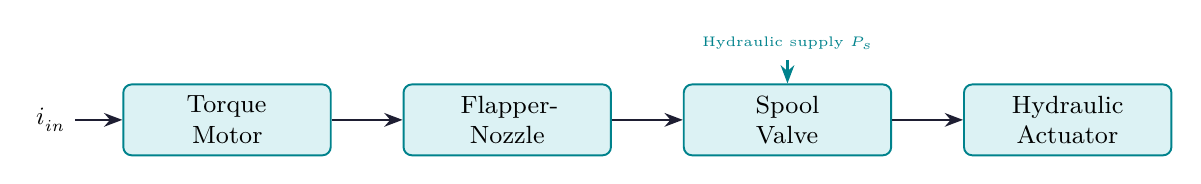
\begin{tikzpicture}[node distance=0.4cm and 1.0cm]
  \node[block] (torque) {Torque\\Motor};
  \node[block, right=0.9cm of torque] (flapper) {Flapper-\\Nozzle};
  \node[block, right=0.9cm of flapper] (spool) {Spool\\Valve};
  \node[block, right=0.9cm of spool] (act) {Hydraulic\\Actuator};
  \node[left=0.6cm of torque, font=\small] {$i_{in}$};
  \draw[arrow] ($(torque.west)-(0.6,0)$) -- (torque.west);
  \draw[arrow] (torque) -- (flapper);
  \draw[arrow] (flapper) -- (spool);
  \draw[arrow] (spool) -- (act);
  \node[above=0.3cm of spool, font=\tiny, color=myteal] {Hydraulic supply $P_s$};
  \draw[arrow,color=myteal] ($(spool.north)+(0,0.3)$) -- (spool.north);
\end{tikzpicture}
\end{tcolorbox}

\subsection{Hydraulic Servomotor}

\begin{tcolorbox}[defbox]
\textbf{Hydraulic Servomotor:} A hydraulic actuator (linear cylinder or rotary motor) that converts \textbf{hydraulic power} (pressure $\times$ flow) into \textbf{mechanical motion}. Controlled by an electro-hydraulic valve.\\[4pt]
\textbf{Advantages:} Very high force/torque output; fast response; high power-to-weight ratio.\\
\textbf{Disadvantages:} Requires hydraulic power supply; risk of leakage; maintenance intensive.
\end{tcolorbox}

\begin{tcolorbox}[formulabox, title={Hydraulic Actuator Transfer Function}]
For a hydraulic cylinder with spool valve:
$$\frac{X(s)}{I(s)} = \frac{K_h}{s(Ms + B)}$$
where $K_h$ = hydraulic gain, $M$ = load mass, $B$ = viscous damping, $X$ = piston displacement, $I$ = input current to valve.
\end{tcolorbox}

\subsection{Electro-Pneumatic Valve}

\begin{tcolorbox}[defbox]
\textbf{Electro-Pneumatic Valve:} Converts an \textbf{electrical signal} into a \textbf{pneumatic pressure or flow}. Used to control pneumatic actuators. Types: I/P converter (current-to-pressure), solenoid valve.\\[4pt]
\textbf{I/P Converter:} Converts 4--20 mA current signal to 3--15 psi (or 0.2--1.0 bar) pneumatic output. Standard interface between electronic controllers and pneumatic actuators in process industries.
\end{tcolorbox}

\subsection{Pneumatic Actuator}

\begin{tcolorbox}[defbox]
\textbf{Pneumatic Actuator:} Converts \textbf{compressed air pressure} into \textbf{mechanical motion} (linear or rotary). Controlled by an electro-pneumatic valve or I/P converter.\\[4pt]
\textbf{Types:}
\begin{itemize}[leftmargin=*, itemsep=2pt, topsep=2pt]
  \item \textbf{Spring-return diaphragm actuator:} Air pressure acts on a diaphragm against a spring. Used for control valves. Fail-safe (spring returns to safe position on air failure).
  \item \textbf{Double-acting cylinder:} Air applied alternately to both sides of a piston for bidirectional motion.
  \item \textbf{Rotary vane actuator:} Converts air pressure to rotary motion (limited angle).
\end{itemize}
\end{tcolorbox}

\begin{tabularx}{\linewidth}{|B{3.0cm}|>{\centering\arraybackslash}X|>{\centering\arraybackslash}X|>{\centering\arraybackslash}X|}
\hline
\multicolumn{1}{|>{\centering\arraybackslash}m{3.0cm}|}{\textbf{Feature}} &
\textbf{\color{myamber}Hydraulic} & \textbf{\color{mygreen}Pneumatic} & \textbf{\color{myteal}Electric} \\
\hline
Power density & Very high & Medium & Medium \\
\hline
Speed & Fast & Very fast & Fast \\
\hline
Precision & High & Moderate & Very high \\
\hline
Maintenance & High (leaks) & Low & Low \\
\hline
Compressibility & Incompressible & Compressible & N/A \\
\hline
Typical use & Heavy machinery & Process valves & Robotics, CNC \\
\hline
\end{tabularx}

%═══════════════════════════════════════════════════════════════════════════════
\newpage
\begin{center}
  {\large\bfseries\color{myred} Quick Revision --- Module 7}\\[3pt]
  {\small\color{mydark} Instrumentation \& Actuators $|$ EC601}
\end{center}
\noindent{\color{myred}\rule{\linewidth}{1.2pt}}\vspace{4pt}

\begin{tcolorbox}[formulabox, title={\textbf{Key Formulas at a Glance}}]
\begin{tabularx}{\linewidth}{B{5.0cm} X}
CRO voltage measurement     & $V_{pk} = n_{div} \times \text{V/div}$ \\[2pt]
CRO time period             & $T = n_{div} \times \text{time/div}$ \\[2pt]
CRO frequency               & $f = 1/T$ \\[2pt]
CRO phase difference        & $\phi = (\Delta t / T)\times 360^\circ$ \\[2pt]
Lissajous phase angle       & $\sin\theta = y_1/y_2$ \\[2pt]
Lissajous frequency ratio   & $f_y/f_x = N_h/N_v$ \\[2pt]
LVDT output                 & $V_{out} = V_{S1} - V_{S2}$; zero at null position \\[2pt]
DC tacho output             & $V_{out} = K_t\,\omega$ \\[2pt]
DC servomotor TF            & $\Omega(s)/V_a(s) = (K_T/R_a)/(Js+B+K_TK_b/R_a)$ \\[2pt]
AC servomotor TF            & $G(s) = K_m/[s(\tau_m s+1)]$ \\[2pt]
Hydraulic actuator TF       & $X(s)/I(s) = K_h/[s(Ms+B)]$ \\[2pt]
I/P converter range         & 4--20 mA $\to$ 3--15 psi (0.2--1.0 bar)
\end{tabularx}
\end{tcolorbox}

\vspace{5pt}

\begin{tcolorbox}[defbox, title={\textbf{One-Line Definitions}}]
\begin{itemize}[leftmargin=*, itemsep=3pt, topsep=0pt]
  \item \textbf{CRO:} Displays voltage vs time waveforms; measures amplitude, frequency, phase, rise time.
  \item \textbf{Trigger circuit:} Synchronises CRO sweep with input signal for stable display.
  \item \textbf{Delay line:} Delays signal in CRO so sweep starts before signal arrives.
  \item \textbf{Lissajous Figure:} Pattern displayed on CRO by two orthogonal sinusoidal signals.
  \item \textbf{Chop Mode:} Switching between channels at high speed; used for low-frequency signals.
  \item \textbf{Alternate Mode:} Switching channels after each sweep; used for high-frequency signals.
  \item \textbf{DSO:} Digital Storage Oscilloscope; digitises, stores, and displays waveforms.
  \item \textbf{Pre-trigger Viewing:} DSO feature to view signal before trigger using circular buffer.
  \item \textbf{Wave analyzer:} Measures amplitude of individual harmonics; narrow tunable BPF.
  \item \textbf{Spectrum analyzer:} Displays full frequency spectrum (amplitude vs frequency) simultaneously.
  \item \textbf{LVDT:} Inductive displacement sensor; output voltage proportional to core displacement.
  \item \textbf{Null position (LVDT):} Core centred; $V_{S1}=V_{S2}$; $V_{out}=0$.
  \item \textbf{DC servomotor:} DC motor for servo use; controlled by armature voltage; linear torque-speed.
  \item \textbf{AC servomotor:} 2-phase induction motor; high rotor resistance; low inertia; drag-cup rotor.
  \item \textbf{Tachogenerator:} Speed-to-voltage transducer; used as velocity feedback sensor.
  \item \textbf{Electro-hydraulic valve:} Converts electrical signal to hydraulic flow; flapper-nozzle type.
  \item \textbf{Hydraulic servomotor:} High-force actuator; converts hydraulic power to mechanical motion.
  \item \textbf{I/P converter:} Converts 4--20 mA to 3--15 psi; interfaces electronic controller to pneumatic actuator.
  \item \textbf{Pneumatic actuator:} Converts compressed air to mechanical motion; spring-return is fail-safe.
\end{itemize}
\end{tcolorbox}

\vspace{5pt}

\begin{tcolorbox}[exambox, title={\textbf{Frequently Asked / Viva Questions}}]
\begin{enumerate}[topsep=0pt, label=\textbf{Q\arabic*.}, itemsep=5pt]
  \item \Q{What is the function of the trigger circuit in a CRO?}
    It synchronises the time base sweep with the input signal so that the waveform appears stationary (stable) on the screen.
  \item \Q{Why is a delay line used in a CRO?}
    To delay the signal slightly so the sweep generator starts before the signal arrives, ensuring the leading edge of the waveform is displayed.
  \item \Q{How do you measure frequency using a CRO?}
    Measure the time period $T$ (horizontal divisions $\times$ time/div for one complete cycle), then $f = 1/T$.
  \item \Q{How can phase difference and frequency ratio be measured using Lissajous figures?}
    Phase difference: for equal frequencies, $\theta = \sin^{-1}(y_1/y_2)$ from the ellipse intercepts. Frequency ratio: for unequal frequencies, $f_y/f_x = N_h/N_v$, where $N_h$ and $N_v$ are horizontal and vertical tangency counts.
  \item \Q{What is the difference between Chop and Alternate modes in a Dual-Trace CRO?}
    Chop mode switches between channels rapidly during a single sweep (best for low frequencies). Alternate mode sweeps Channel A completely, then Channel B on the next sweep (best for high frequencies to prevent trace flicker).
  \item \Q{What is the main advantage of a DSO over an analog CRO?}
    DSOs digitise and store signals in digital memory, offering infinite waveform storage, pre-trigger viewing (circular buffer recording), and built-in microprocessor-based signal processing.
  \item \Q{How does a DSO achieve pre-trigger viewing?}
    It continuously writes ADC samples to a circular memory buffer. When the trigger occurs, it stops writing after a specific delay, retaining the samples that were stored prior to the trigger event.
  \item \Q{What is the difference between a wave analyzer and a spectrum analyzer?}
    Wave analyzer measures one frequency component at a time (narrow tunable BPF). Spectrum analyzer displays all frequency components simultaneously on screen.
  \item \Q{What is LVDT and how does it work?}
    Linear Variable Differential Transformer. AC excitation on primary induces EMF in two secondary coils connected in series opposition. Output voltage is proportional to core displacement; zero at null position.
  \item \Q{What is the output of LVDT at null position?}
    Zero, because the two secondary voltages are equal and opposite ($V_{S1} = V_{S2}$, so $V_{out} = V_{S1} - V_{S2} = 0$).
  \item \Q{What are the advantages of LVDT?}
    Infinite resolution (frictionless/contactless), high accuracy, no mechanical wear, rugged, works in harsh environments.
  \item \Q{What is the difference between DC and AC servomotor?}
    DC: controlled by armature voltage, uses brushes, high power. AC: 2-phase induction, brushless, high rotor resistance for linear torque-speed, low inertia drag-cup rotor.
  \item \Q{What is a tachogenerator?}
    A speed transducer that generates a voltage proportional to rotational speed ($V = K_t\omega$). Used as velocity feedback in closed-loop speed control.
  \item \Q{What is an electro-hydraulic servo valve?}
    Converts electrical current to hydraulic flow using a torque motor, flapper-nozzle, and spool valve. Controls hydraulic actuator position/speed.
  \item \Q{What is an I/P converter?}
    Current-to-pressure converter. Converts 4--20 mA electrical signal to 3--15 psi pneumatic signal. Standard interface between electronic controllers and pneumatic actuators.
  \item \Q{Why is a spring-return pneumatic actuator called fail-safe?}
    On loss of air supply, the spring returns the actuator (and connected valve) to a predetermined safe position (fully open or fully closed).
\end{enumerate}
\end{tcolorbox}

\end{document}
